\documentclass[aspectratio=169]{beamer}


\usepackage[brazil]{babel}
\usepackage[utf8]{inputenc}
\usepackage{algorithm, algpseudocode}
\usepackage{graphicx}
\usepackage{subfig}
\usepackage[absolute]{textpos}
\makeatletter
\renewcommand{\ALG@beginalgorithmic}{\small}
\makeatother

\usetheme[progressbar=foot]{metropolis}

\title{Projeto e Análise de Algoritmos}
\subtitle{Caminhos Mínimos Utilizando Algoritmos de Dijkstra, Bellman-Ford, Floyd-Warshall, com detecção de Ciclos de Custo Negativo}
\date{\today}
\author{Conrado C. Bicalho, Danilo S. Souza, Rodolfo L. M. Guimarães, Thiago Schons}

\institute{
	\textit{\{conradobh, danilo.gdc, rodolfolabiapari, thiagoschons2\}@gmail.com} \\
	Departamento de Computação -- Universidade Federal de Ouro Preto \\
		35.400-000 -- Ouro Preto - MG -- Brasil 
	}



\begin{document}
	\maketitle
  
  
\usebackgroundtemplate{
\includegraphics[trim=0 245cm 0 0, width=0.05\textwidth]{img/ufop.jpg}}
  
\section{Introdução}
	\begin{frame}{Teoria dos Grafos}
		\begin{itemize}
			\item {\footnotesize 	
				Estrutura $G=(V,E)$ onde  \cite{netto2003grafos}:
				\begin{itemize}
					\item $V$ é um conjunto discreto e não vazio de vértices;
					\item $E$ é uma família de elementos não vazios definidos em função dos elementos em $V$.
					
					Cada aresta tem um ou dois nós associados a ela e faz o papel de interligar suas extremidades.
				\end{itemize} 
				
			
			\item No grafo orientado cada aresta orientada está associada a um par ordenado de nós $(u, v)$.
		}
			\begin{figure}[!htb]
				\centering
					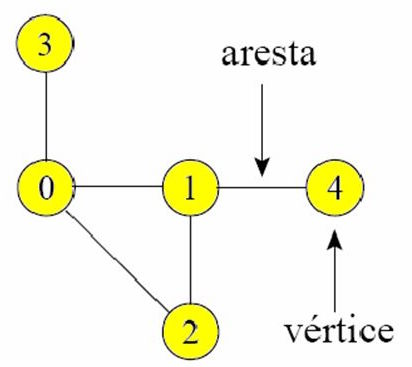
\includegraphics[width=0.25\textwidth]{img/naoponderado.jpg}
					%\caption{}
					\label{fig:naoponderado}
				\quad \quad 
					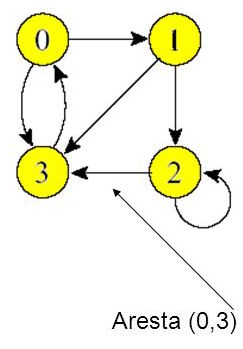
\includegraphics[width=0.18\textwidth]{img/ponderado.jpg}
					%	\caption{ }
					\label{fig:orientado}
				
			%	\caption{Fonte: Autor.}
				\label{fig01}
			\end{figure}
			{\footnotesize 
			\item Tais arcos também podem ser ponderados sendo sua função peso $w(u, v) : E \rightarrow \mathbb{R}$ \cite{netto2003grafos}.}
		\end{itemize}
	\end{frame}

\section{Definição do Problema}
	\begin{frame}{Definição do Problema de Caminhos Mínimos de Única Origem \cite{cormen2002algoritmos}} 
			
		\begin{itemize}
			\item Grafo $G = (V, E)$ sem laços e valorado por uma função peso $w : E \rightarrow \mathbb{R}$, sendo o peso $p = \left \langle v_{1}, v_{2}, \ldots, v_{k}  \right \rangle$ onde o somatório dos pesos de suas arestas
		
			$$w(p) = \sum_{i=1}^{k} w(v_{i-1}, v_{i})$$
			
			\item Assim, o peso do caminho mais curto de $u$ até $v$ é 
		
			$$
			\delta(u, v) = 
			\begin{cases}
			\text{min}\{w(p):u\xrightarrow{p} v\} & \text{se existe um caminho de } u \text{ até } v\text{,}\\
			\infty & \text{em caso contrário.}
			\end{cases}
			$$
			
			\item Propriedade de que:
			\begin{itemize}
				\item  Um caminho mais curto entre dois vértices pode conter outros caminhos mais curtos em seu interior.
			\end{itemize}
		\end{itemize}
	\end{frame}
	
	
	\begin{frame}{Caminhos mais Curtos de Todos para Todos}
		\begin{itemize}
			\item Deseja-se encontrar o caminho mais curto entre todos os pares de vértices $u,v \in V$. 
			
			\bigskip
			
			\item Este problema também pode ser resolvido utilizando um algoritmo de caminho mínimo um para todos $|V|$ vezes, uma para cada vértice de origem:
			\begin{itemize}
				\item Mas existem algoritmos específicos para a resolução deste.
			\end{itemize}
			
			\bigskip
			
			\item Sua estrutura de dados é lidada como uma matriz de adjacência:
			\begin{itemize}
				\item  É exibido os valores de todos para todos de acordo com sua linha e colina.
			\end{itemize}
		\end{itemize}
	\end{frame}
	
	
	\begin{frame}{Caminhos mais Curtos de Todos para Todos}
		\begin{itemize}
			\item Supondo que existem $|V|$ vértices e enumerados de forma crescente e contínua, uma matriz de entrada seria $W\ n \times n$ representando os peso das arestas do grafo orientado de $n$ vértices. Isto é, $W = (w_{ij})$ onde 
		\end{itemize}
		
		$$
		w_{ij} = 
		\begin{cases}
		0 & \mbox{se } i = j, \\
		\mbox{o peso da aresta orientada } (i, j) & \mbox{se } i \neq j \mbox{ e } (i, j) \in E, \\
		\infty & \mbox{se } i \neq j \mbox{ e } (i, j) \notin E.
		\end{cases}
		$$
		
		\bigskip
		
		$$
		\forall\delta(u, v) = 
		\begin{cases}
		\text{min}\{w(p):u\xrightarrow{p} v\} & \text{se existe um caminho de } u \text{ até } v\text{,}\\
		\infty & \text{em caso contrário.}
		\end{cases}
		$$
		
	\end{frame}

\section{Prova}
	\begin{frame}{Subestrutura Ótima de um Caminho Mais Curto \cite{cormen2002algoritmos}}
		\begin{itemize}
			\item \textit{\textbf{Lema:}}
			\begin{itemize}
				\item Dado um grafo orientado ponderado $G = (V, E)$ com função peso $w : E \rightarrow \mathbb{R}$, seja $p = \left \langle v_{1}, v_{2}, \ldots, v_{k}\right \rangle$ um caminho mais curto.
				
				\item Para quaisquer $i$ e $j$ tais que $1 \le i \le j \le k$, seja $p_{ij}= \left \langle v_{i}, v_{i + 1}, \ldots, v_{j}\right \rangle$ o subcaminho. 
				
				\item Então, $p_{ij}$ é um caminho mais curto de $v_i$ e $v_j$.
			\end{itemize}
			
			\bigskip
			\pause
			
			\item \textit{\textbf{Prova:}}
			\begin{itemize}
				\item  Quando decompõe o caminho $p$ em $v_1 \xrightarrow{p_{1i}} v_i \xrightarrow{p_{ij}} v_j \xrightarrow{p_{jk}} v_k$, teremos $w(p) = w(p_{1i}) + w(p_{ij}) + w(p_{jk})$. 
				
				\item Supondo que existisse um caminho $p^\prime_{ij}$ de $v_i$ até $v_j$ com peso $w(p^\prime_{ij}) < w(p_{ij})$. 
				
				\item Então, $v_1 \xrightarrow{p_{1i}} v_i \xrightarrow{p^\prime_{ij}} v_j \xrightarrow{p_{jk}} v_k$ é um caminho de $v_1$ até $v_k$ cujo peso $w(p) = w(p_{1i}) + w(p^\prime_{ij}) + w(p_{jk})$ é menor que $w(p)$, o que \textbf{contradiz a hipótese de que $p$ é um caminho mais curto de $v_1$ até $v_k$}.
			\end{itemize}
		\end{itemize}
	\end{frame}
	

\section{Itens Importantes}
	\begin{frame}{Arestas de Peso Negativo}
		\begin{itemize}
			\item Em algumas instâncias do problema, pode haver arestas cujo pesos são negativos. 
		\end{itemize}
		
			\begin{figure}[H]
				\centering
				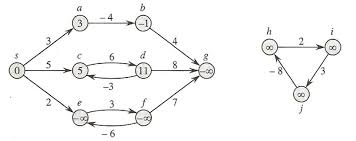
\includegraphics[width=0.8\textwidth]{img/negativo2.jpeg}
				\caption{Exemplo simples de um grafo com arestas de peso negativo. Fonte: \cite{cormen2002algoritmos}.}
				\label{fig:negativo1}
			\end{figure}
	\end{frame}
	
	
	\begin{frame}{Arestas de Peso Negativo}
		\begin{figure}[H]
			\centering
			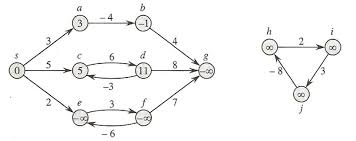
\includegraphics[width=0.6\textwidth]{img/negativo2.jpeg}
			%\caption{Exemplo simples de um grafo com arestas de peso negativo. Fonte: \cite{cormen2002algoritmos}.}
			\label{fig:negativo}
		\end{figure}
		
		\begin{itemize}
			\item Um grafo $G = (V,E)$ que não contenha nenhum ciclo de peso negativo acessível a partir da origem $s$:
			\begin{itemize}
				\item  $\forall v \in V$, o peso do caminho mais curto $\delta(s,v)$ permanece \textbf{bem definido}, mesmo tendo um valor negativo. 
				
				\pause
				
				\item Mas, caso exista um ciclo de peso negativo acessível, os pesos dos caminhos \textbf{não serão bem definidos}:
				\begin{itemize}
					\item Existindo o ciclo negativo no caminho de $s$ até $v$, então $\delta(s,v) = - \infty$ \cite{cormen2002algoritmos}. 
				\end{itemize}
			\end{itemize}
		\end{itemize}
	\end{frame}
	
	
\section{Algoritmos}
	
	\begin{frame}{Ambiente de Hardware e Software Utilizado}
		\begin{table}[H]
			\caption{Tabela com as informações de ambiente de execução do trabalho realizado.}
			\centering
			\begin{tabular}{l|l}
				\hline
				\textbf{Item}                & \textbf{Descrição} \\ \hline \hline
				Processador         & 1 Processador Intel Core i7 - 2,9 GHz         \\
				Núcleos             & 4 Núcleos \\
				Cache L2 (por Núcleo) & 256 KB \\
				Cache L3            & 4 MB \\
				Memória RAM         & 10 GB DDR3        \\
				Arquitetura         & Arquitetura de von Neumann         \\
				Sistema Operacional & OS X 10.11.4 (15E65)         \\
				Versão do Kernel    & Darwin 15.4.0 \\
				Compilador          & Apple LLVM version 7.3.0 (clang-703.0.31)         \\\hline
			\end{tabular}
		\end{table}
	\end{frame}
	
\subsection{Bellman Ford}
	\begin{frame}{Algoritmo Bellman-Ford}
		\begin{algorithm}[H]
			\caption{Bellman-Ford}\label{alg:d}
			\begin{algorithmic}[1]
				\Procedure{Bellman-Ford}{$G, w, s$}
				\State INICIALIZA-UNICA-FONTE(G, s);
				\For{$i \gets 1, |V[G]| - 1$}   
				\For{cada aresta $(u,v) \in E[G]$} 
				\State RELAXA(u, v, w);  
				\EndFor
				\EndFor
				
				\For{cada aresta $(u,v) \in E[G]$}
				\If{$d[v] > d[u] + w(u,v)$}   
				\State \textbf{return} FALSE;
				\EndIf
				\EndFor
				\State \textbf{return} TRUE;
				\EndProcedure
			\end{algorithmic}
		\end{algorithm}
	\end{frame}
	
	\begin{frame}{Algoritmo Bellman-Ford}
		\begin{algorithm}[H]
			\caption{Bellman-Ford}\label{alg:d}
			\begin{algorithmic}[1]
				\Procedure{Bellman-Ford}{$G, w, s$}
				\State INICIALIZA-UNICA-FONTE(G, s);
				\For{$i \gets 1, |V[G]| - 1$}   \Comment{$\mathcal{O}(V)$}
				\For{cada aresta $(u,v) \in E[G]$} 
				\State RELAXA(u, v, w);   
				\EndFor
				\EndFor
				
				\For{cada aresta $(u,v) \in E[G]$}
				\If{$d[v] > d[u] + w(u,v)$}   
				\State \textbf{return} FALSE;
				\EndIf
				\EndFor
				\State \textbf{return} TRUE;
				\EndProcedure
			\end{algorithmic}
		\end{algorithm}
	\end{frame}
	
	\begin{frame}{Algoritmo Bellman-Ford}
		\begin{algorithm}[H]
			\caption{Bellman-Ford}\label{alg:d}
			\begin{algorithmic}[1]
				\Procedure{Bellman-Ford}{$G, w, s$}
				\State INICIALIZA-UNICA-FONTE(G, s);
				\For{$i \gets 1, |V[G]| - 1$}   \Comment{$\mathcal{O}(V)$}
				\For{cada aresta $(u,v) \in E[G]$} \Comment{$\mathcal{O}(E)$}  
				\State RELAXA(u, v, w);   
				\EndFor
				\EndFor
				
				\For{cada aresta $(u,v) \in E[G]$}
				\If{$d[v] > d[u] + w(u,v)$}   
				\State \textbf{return} FALSE;
				\EndIf
				\EndFor
				\State \textbf{return} TRUE;
				\EndProcedure
			\end{algorithmic}
		\end{algorithm}
	\end{frame}
	
	\begin{frame}{Algoritmo Bellman-Ford}
		\begin{algorithm}[H]
			\caption{Bellman-Ford}\label{alg:d}
			\begin{algorithmic}[1]
				\Procedure{Bellman-Ford}{$G, w, s$}
				\State INICIALIZA-UNICA-FONTE(G, s);
				\For{$i \gets 1, |V[G]| - 1$}   \Comment{$\mathcal{O}(V)$}
				\For{cada aresta $(u,v) \in E[G]$} \Comment{$\mathcal{O}(E)$}  
				\State RELAXA(u, v, w);   \Comment{$\mathcal{O}(1)$}
				\EndFor
				\EndFor
				
				\For{cada aresta $(u,v) \in E[G]$}
				\If{$d[v] > d[u] + w(u,v)$}  
				\State \textbf{return} FALSE;
				\EndIf
				\EndFor
				\State \textbf{return} TRUE;
				\EndProcedure
			\end{algorithmic}
		\end{algorithm}
	\end{frame}
	
	
	\begin{frame}{Algoritmo Bellman-Ford}
		\begin{algorithm}[H]
			\caption{Bellman-Ford}\label{alg:d}
			\begin{algorithmic}[1]
				\Procedure{Bellman-Ford}{$G, w, s$}
				\State INICIALIZA-UNICA-FONTE(G, s);
				\For{$i \gets 1, |V[G]| - 1$}   \Comment{$\mathcal{O}(V)$}
				\For{cada aresta $(u,v) \in E[G]$} \Comment{$\mathcal{O}(E)$}  
				\State RELAXA(u, v, w);   \Comment{$\mathcal{O}(1)$}
				\EndFor
				\EndFor
				
				\For{cada aresta $(u,v) \in E[G]$} \Comment{$\mathcal{O}(E)$}
				\If{$d[v] > d[u] + w(u,v)$}   
				\State \textbf{return} FALSE;
				\EndIf
				\EndFor
				\State \textbf{return} TRUE;
				\EndProcedure
			\end{algorithmic}
		\end{algorithm}
	\end{frame}
	
	\begin{frame}{Algoritmo Bellman-Ford}
		\begin{algorithm}[H]
			\caption{Bellman-Ford}\label{alg:d}
			\begin{algorithmic}[1]
				\Procedure{Bellman-Ford}{$G, w, s$}
				\State INICIALIZA-UNICA-FONTE(G, s);
				\For{$i \gets 1, |V[G]| - 1$}   \Comment{$\mathcal{O}(V)$}
				\For{cada aresta $(u,v) \in E[G]$} \Comment{$\mathcal{O}(E)$}  
				\State RELAXA(u, v, w);   \Comment{$\mathcal{O}(1)$}
				\EndFor
				\EndFor
				
				\For{cada aresta $(u,v) \in E[G]$} \Comment{$\mathcal{O}(E)$}
				\If{$d[v] > d[u] + w(u,v)$}   \Comment{$\mathcal{O}(1)$}
				\State \textbf{return} FALSE;
				\EndIf
				\EndFor
				\State \textbf{return} TRUE;
				\EndProcedure
			\end{algorithmic}
		\end{algorithm}
	\end{frame}
	
\section{Algoritmo de Dijkstra}
	\begin{frame}{Algoritmo de Dijkstra}
		\begin{algorithm}[H]
			\caption{Dijkstra}\label{alg:d}
			\begin{algorithmic}[1]
				\Procedure{Dijkstra}{$G, w, s$}
				\State INICIALIZA-UNICA-FONTE(G, s);
				\State $S\gets \emptyset$;
				\State $Q\gets V[G]$;
				\While{$Q\not=\emptyset$}
				\State $u\gets$ RETIRA-MINIMO(Q);
				\State $S\gets S \cup \{u\}$;
				\For{cada vértice vizinho $v \in Adj[u]$}
				\State RELAXA(u, v, w);
				\EndFor
				\EndWhile\label{euclidendwhile}
				\EndProcedure
			\end{algorithmic}
		\end{algorithm}
	\end{frame}
	
	\begin{frame}{Algoritmo de Dijkstra}
		\begin{algorithm}[H]
			\caption{Dijkstra}\label{alg:d}
			\begin{algorithmic}[1]
				\Procedure{Dijkstra}{$G, w, s$}
				\State INICIALIZA-UNICA-FONTE(G, s);               \Comment{$\mathcal{O}(E)$}
				\State $S\gets \emptyset$;
				\State $Q\gets V[G]$;
				\While{$Q\not=\emptyset$}                      
				\State $u\gets$ RETIRA-MINIMO(Q);              
				\State $S\gets S \cup \{u\}$;
				\For{cada vértice vizinho $v \in Adj[u]$}             
				\State RELAXA(u, v, w);
				\EndFor
				\EndWhile\label{euclidendwhile}
				\EndProcedure
			\end{algorithmic}
		\end{algorithm}
	\end{frame}
	
	\begin{frame}{Algoritmo de Dijkstra}
		\begin{algorithm}[H]
			\caption{Dijkstra}\label{alg:d}
			\begin{algorithmic}[1]
				\Procedure{Dijkstra}{$G, w, s$}
				\State INICIALIZA-UNICA-FONTE(G, s);               \Comment{$\mathcal{O}(E)$}
				\State $S\gets \emptyset$;
				\State $Q\gets V[G]$;
				\While{$Q\not=\emptyset$}                       \Comment{$\mathcal{O}(V)$}
				\State $u\gets$ RETIRA-MINIMO(Q);               
				\State $S\gets S \cup \{u\}$;
				\For{cada vértice vizinho $v \in Adj[u]$}              
				\State RELAXA(u, v, w);
				\EndFor
				\EndWhile\label{euclidendwhile}
				\EndProcedure
			\end{algorithmic}
		\end{algorithm}
	\end{frame}
	
	\begin{frame}{Algoritmo de Dijkstra}
		\begin{algorithm}[H]
			\caption{Dijkstra}\label{alg:d}
			\begin{algorithmic}[1]
				\Procedure{Dijkstra}{$G, w, s$}
				\State INICIALIZA-UNICA-FONTE(G, s);               \Comment{$\mathcal{O}(E)$}
				\State $S\gets \emptyset$;
				\State $Q\gets V[G]$;
				\While{$Q\not=\emptyset$}                       \Comment{$\mathcal{O}(V)$}
				\State $u\gets$ RETIRA-MINIMO(Q);               \Comment{$\mathcal{O}(1)$}
				\State $S\gets S \cup \{u\}$;
				\For{cada vértice vizinho $v \in Adj[u]$}              
				\State RELAXA(u, v, w);
				\EndFor
				\EndWhile\label{euclidendwhile}
				\EndProcedure
			\end{algorithmic}
		\end{algorithm}
	\end{frame}
	
	\begin{frame}{Algoritmo de Dijkstra}
		\begin{algorithm}[H]
			\caption{Dijkstra}\label{alg:d}
			\begin{algorithmic}[1]
				\Procedure{Dijkstra}{$G, w, s$}
				\State INICIALIZA-UNICA-FONTE(G, s);               \Comment{$\mathcal{O}(E)$}
				\State $S\gets \emptyset$;
				\State $Q\gets V[G]$;
				\While{$Q\not=\emptyset$}                       \Comment{$\mathcal{O}(V)$}
				\State $u\gets$ RETIRA-MINIMO(Q);               \Comment{$\mathcal{O}(1)$}
				\State $S\gets S \cup \{u\}$;
				\For{cada vértice vizinho $v \in Adj[u]$}               \Comment{$\mathcal{O}(\log V)$}
				\State RELAXA(u, v, w);
				\EndFor
				\EndWhile\label{euclidendwhile}
				\EndProcedure
			\end{algorithmic}
		\end{algorithm}
	\end{frame}
	
	\begin{frame}{Algoritmo de Dijkstra}
		\begin{algorithm}[H]
			\caption{Dijkstra}\label{alg:d}
			\begin{algorithmic}[1]
				\Procedure{Dijkstra}{$G, w, s$}
				\State INICIALIZA-UNICA-FONTE(G, s);               \Comment{$\mathcal{O}(E)$}
				\State $S\gets \emptyset$;
				\State $Q\gets V[G]$;
				\While{$Q\not=\emptyset$}                       \Comment{$\mathcal{O}(V)$}
				\State $u\gets$ RETIRA-MINIMO(Q);               \Comment{$\mathcal{O}(1)$}
				\State $S\gets S \cup \{u\}$;
				\For{cada vértice vizinho $v \in Adj[u]$}               \Comment{$\mathcal{O}(\log V)$}
				\State RELAXA(u, v, w);                                   \Comment{$\mathcal{O}(1)$}
				\EndFor
				\EndWhile\label{euclidendwhile}
				\EndProcedure
			\end{algorithmic}
		\end{algorithm}
	\end{frame}
	
	
\section{Algoritmo Floyd Warshall}
	\begin{frame}{Algoritmo Floyd Warshall}
		\begin{algorithm}[H]
			\caption{Floyd-Warshall}\label{alg:fw}
			\begin{algorithmic}[1]
				\Procedure{Floyd-Warshall}{$W$}
				\State $n \gets linhas[W]$;
				\State $D\gets W$;
				\For{$k \gets 1, n$}
				\For{$i \gets 1, n$}
				\For{$j \gets 1, n$}
				\State $d^k_{ij} \gets min(d^{k-1}_{ij}, d^{k-1}_{ik} + d^{k-1}_{kj})$;
				\EndFor
				\EndFor
				\EndFor
				\State \textbf{return} $D$;
				\EndProcedure
			\end{algorithmic}
		\end{algorithm}
	\end{frame}
	
	\begin{frame}{Algoritmo Floyd Warshall}
		\begin{algorithm}[H]
			\caption{Floyd-Warshall}\label{alg:fw}
			\begin{algorithmic}[1]
				\Procedure{Floyd-Warshall}{$W$}
				\State $n \gets linhas[W]$;
				\State $D\gets W$;
				\For{$k \gets 1, n$}          \Comment{$\mathcal{O}(V)$}
				\For{$i \gets 1, n$}          
				\For{$j \gets 1, n$}         
				\State $d^k_{ij} \gets min(d^{k-1}_{ij}, d^{k-1}_{ik} + d^{k-1}_{kj})$; 
				\EndFor
				\EndFor
				\EndFor
				\State \textbf{return} $D$;
				\EndProcedure
			\end{algorithmic}
		\end{algorithm}
	\end{frame}
	
	\begin{frame}{Algoritmo Floyd Warshall}
		\begin{algorithm}[H]
			\caption{Floyd-Warshall}\label{alg:fw}
			\begin{algorithmic}[1]
				\Procedure{Floyd-Warshall}{$W$}
				\State $n \gets linhas[W]$;
				\State $D\gets W$;
				\For{$k \gets 1, n$}          \Comment{$\mathcal{O}(V)$}
				\For{$i \gets 1, n$}          \Comment{$\mathcal{O}(V)$}
				\For{$j \gets 1, n$}          
				\State $d^k_{ij} \gets min(d^{k-1}_{ij}, d^{k-1}_{ik} + d^{k-1}_{kj})$; 
				\EndFor
				\EndFor
				\EndFor
				\State \textbf{return} $D$;
				\EndProcedure
			\end{algorithmic}
		\end{algorithm}
	\end{frame}
	
	\begin{frame}{Algoritmo Floyd Warshall}
		\begin{algorithm}[H]
			\caption{Floyd-Warshall}\label{alg:fw}
			\begin{algorithmic}[1]
				\Procedure{Floyd-Warshall}{$W$}
				\State $n \gets linhas[W]$;
				\State $D\gets W$;
				\For{$k \gets 1, n$}          \Comment{$\mathcal{O}(V)$}
				\For{$i \gets 1, n$}          \Comment{$\mathcal{O}(V)$}
				\For{$j \gets 1, n$}          \Comment{$\mathcal{O}(V)$}
				\State $d^k_{ij} \gets min(d^{k-1}_{ij}, d^{k-1}_{ik} + d^{k-1}_{kj})$; 
				\EndFor
				\EndFor
				\EndFor
				\State \textbf{return} $D$;
				\EndProcedure
			\end{algorithmic}
		\end{algorithm}
	\end{frame}
	
	\begin{frame}{Algoritmo Floyd Warshall}
		\begin{algorithm}[H]
			\caption{Floyd-Warshall}\label{alg:fw}
			\begin{algorithmic}[1]
				\Procedure{Floyd-Warshall}{$W$}
				\State $n \gets linhas[W]$;
				\State $D\gets W$;
				\For{$k \gets 1, n$}          \Comment{$\mathcal{O}(V)$}
				\For{$i \gets 1, n$}          \Comment{$\mathcal{O}(V)$}
				\For{$j \gets 1, n$}          \Comment{$\mathcal{O}(V)$}
				\State $d^k_{ij} \gets min(d^{k-1}_{ij}, d^{k-1}_{ik} + d^{k-1}_{kj})$;  \Comment{$\mathcal{O}(1)$}
				\EndFor
				\EndFor
				\EndFor
				\State \textbf{return} $D$;
				\EndProcedure
			\end{algorithmic}
		\end{algorithm}
	\end{frame}

\section{Experimentos}
	\begin{frame}{Experimentos}
		\begin{itemize}
			
			\item Realizou-se teste de todos para todos.
			
			\bigskip
						
			\item Utilizou-se de 4 instâncias:
			\begin{itemize}
				\item \textit{rome99.gr}, \textit{rg300\_4730.gr}, \textit{rg300\_768\_floyd.gr}, \textit{rg300\_768\_floyd-n.gr}.
			\end{itemize}
			
			\bigskip
			
			\item Para cada instância foi executado 20 vezes no mesmo ambiente de testes e colhido o tempo de execução.
			
			\bigskip
			
			\item Todos os resultados estão disponíveis no relatório deste trabalho.
		\end{itemize}
	\end{frame}
	
	\begin{frame}{Valores de Tempos de Execução}
		\begin{table}[H]
			\centering
			\caption{Tabela com os valores de tempo médio de cada algoritmo nas quatro instâncias com o objetivo de obter caminhos mínimos de todos para todos.}
			{\footnotesize 
			
			\begin{tabular}{l|lll}
				\hline
				\textbf{Instância} & \textbf{Bellman-Ford (s)} & \textbf{Dijkstra (s)} & \textbf{Ford-Warshall (s)} \\ \hline \hline
				\textit{ rome99.gr}         & 420.0757                           & 93.59347                          & 149.3292                            \\
				\textit{ rg300\_4730.gr}         & 1.788467                           & 0.11464                          & 0.118966                            \\
				\textit{ rg300\_768\_floyd.gr}         & 0.294253                           & 0.094997                          & 0.116002                            \\
				\textit{ rg300\_768\_floyd-n.gr}    & 0.289948  & Não se aplica.                              & 0.098479                            \\ \hline
			\end{tabular}	
			}
		\end{table}
	\end{frame}
	
	
	\begin{frame}{}
		\begin{itemize}
			\item A Figura \ref{fig:rome} exibe um gráfico comparando os resultados de cada algoritmo sobre a instância \textit{rome99.gr}.
			
			\begin{figure}[H]
				\centering
				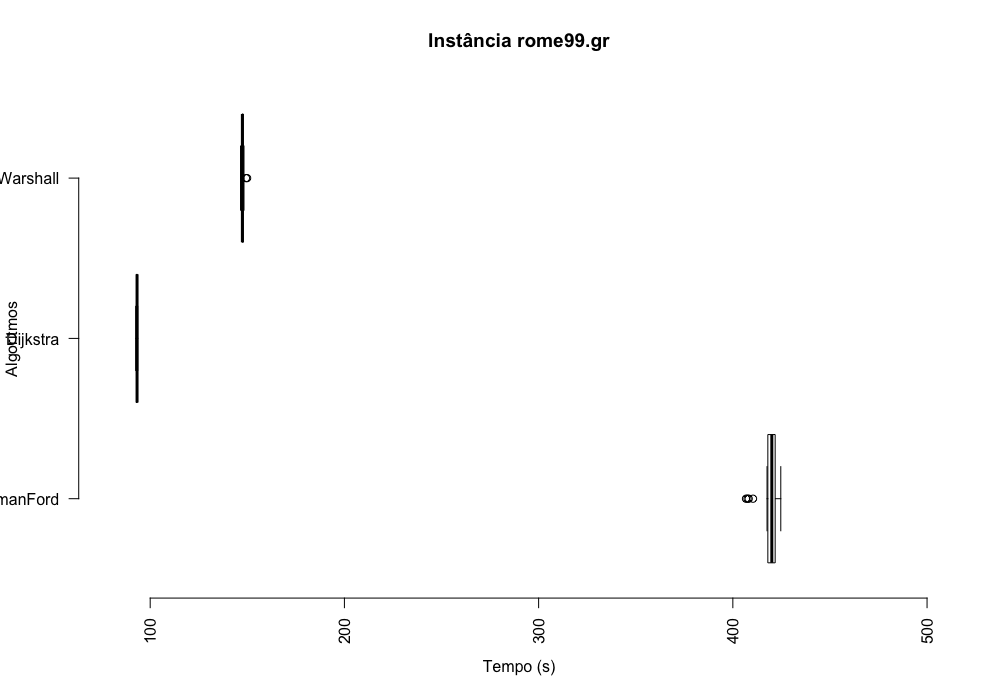
\includegraphics[width=0.8\textwidth]{img/rome99.png}
				\caption{Tempo de execução de cada algoritmo sobre a instância \textit{rome99.gr}. Fonte: Autor.}
				\label{fig:rome}
			\end{figure}
		\end{itemize}
	\end{frame}
	
	\begin{frame}{}
		\begin{itemize}
			\item A Figura \ref{fig:rg300_4730} exibe um gráfico comparando os resultados de cada algoritmo sobre a instância \textit{ rg300\_4730.gr}.
			
			\begin{figure}[H]
				\centering
				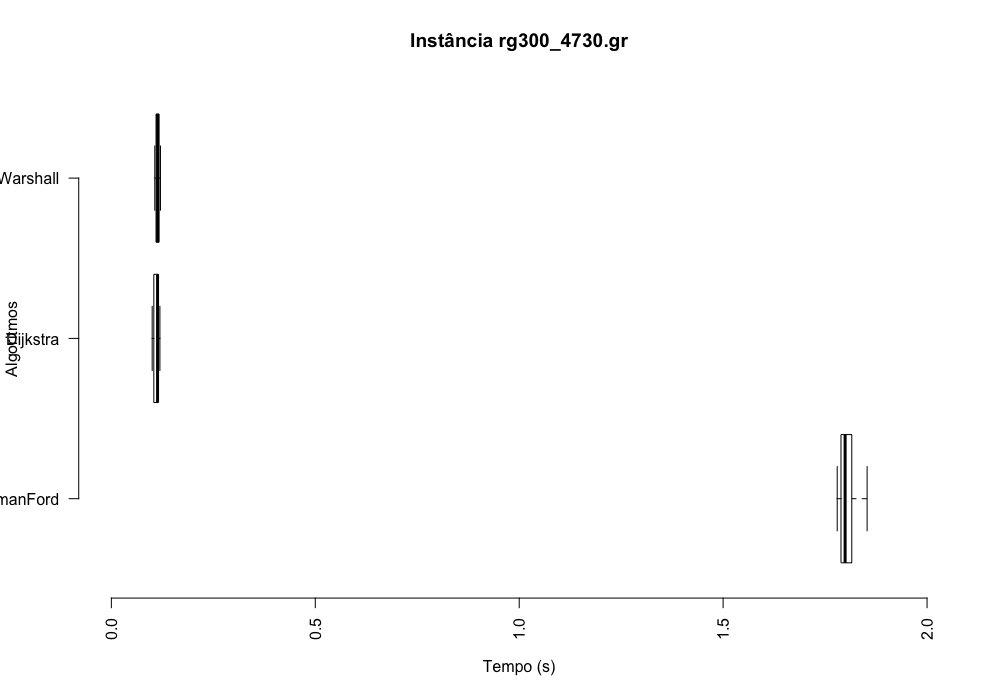
\includegraphics[width=0.8\textwidth]{img/rg300_4730.png}
				\caption{Tempo de execução de cada algoritmo sobre a instância \textit{rg300\_4730.gr}. Fonte: Autor.}
				\label{fig:rg300_4730}
			\end{figure}
		\end{itemize}
	\end{frame}
	
	\begin{frame}{}
		\begin{itemize}
			\item A Figura \ref{fig:rg300_768_floyd} exibe um gráfico comparando os resultados de cada algoritmo sobre a instância \textit{ rg300\_768\_floyd.gr}.
			
			\begin{figure}[H]
				\centering
				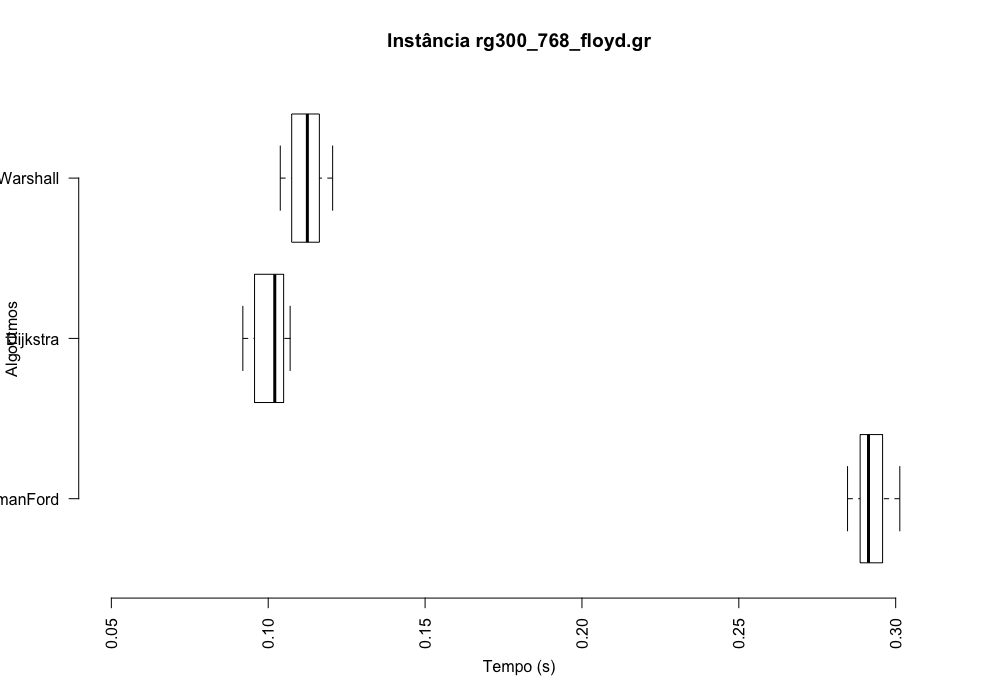
\includegraphics[width=0.8\textwidth]{img/rg300_768_floyd.png}
				\caption{Tempo de execução de cada algoritmo sobre a instância \textit{rg300\_768\_floyd.gr}. Fonte: Autor.}
				\label{fig:rg300_768_floyd}
			\end{figure}
		\end{itemize}
	\end{frame}
	
	\begin{frame}{}
		\begin{itemize}
			\item A Figura \ref{fig:rg300_768_floyd_n} exibe um gráfico comparando os resultados de cada algoritmo sobre a instância \textit{ rg300\_768\_floyd-n.gr}.
			
			\begin{figure}[H]
				\centering
				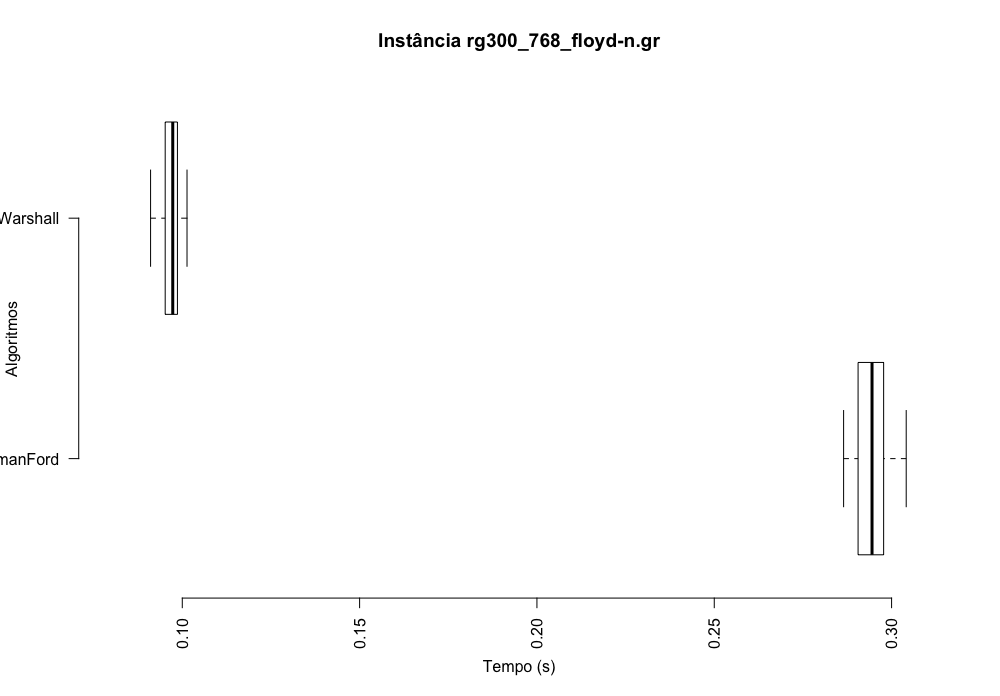
\includegraphics[width=0.8\textwidth]{img/rg300_768_floyd-n_gr.png}
				\caption{Tempo de execução de cada algoritmo sobre a instância com arestas negativas \textit{rg300\_768\_floyd-n.gr}. Fonte: Autor.}
				\label{fig:rg300_768_floyd_n}
			\end{figure}
		\end{itemize}
	\end{frame}
	
\section{Conclusão}
	\begin{frame}{Conclusão}
		\begin{itemize}
			\item O problema de caminhos mínimos também está relacionado a programação linear:
			\begin{itemize}
				\item É possível reduzir um caso especial de programação linear ao fato de encontrar caminhos mais curtos a partir de uma única origem.
				
				\item Tal problema pode ser resolvido com algoritmo de Bellman-Ford, sendo assim resolvendo também o problema de programação linear \cite{cormen2002algoritmos}.
			\end{itemize}
			
			\bigskip
			
			\item Realizou-se 20 iterações de teste por ser uma média razoável para análise e também devido ao tempo computacional elevado pelo tamanho das instâncias utilizadas assim como a complexidade dos algoritmos. 
			
		\end{itemize}
	\end{frame}
	
	\begin{frame}{Conclusão}
		\begin{itemize}
			\item Em termos de implementação:
			\begin{itemize}
				\item Todos os códigos possuem grande facilidade de implementação:
				
				\item Principalmente o Algoritmo Floyd-Warshall.
			\end{itemize}
			
			\bigskip
			
			\item Sobre a análise assintótica:
			\begin{itemize}
				\item Houve uma grande disputa entre o Bellman-Ford e Dijkstra. 
				
				\item O Algoritmo de Floyd-Warshall ficou fora dessa disputa por ser de complexidade de tempo  $\mathcal{O}(n^3)$
				
				\item E o Bellman tem complexidade  $\mathcal{O}(n^2)$ e o Dijkstra $\mathcal{O}(E + V \log V)$ no pior caso. 
				
				\item O Algoritmo Dijkstra teve sucesso em todas as execuções devida sua complexidade assintótica de tempo ser menor que todos os outros $\mathcal{O}(E + V \log V) < \mathcal{O}(n^2)$.
			\end{itemize}
		\end{itemize}
	\end{frame}


\section{Bibliografia}

\bibliographystyle{abbrv}
\bibliography{sbc-template}

\maketitle


\begin{frame}{Considerações de Projeto e Análise}
	
	\begin{itemize}
		\item Alguns algoritmos implementados tratam o `infinito' como: o maior peso encontradas das arestas multiplicado por ele mesmo.
		
		\bigskip
		
		\item A estrutura utilizada no Algoritmo de Dijkstra foi projetada pelos integrantes dos grupos.
		
		\bigskip
		
		\item Nenhum algoritmo faz teste de verificação de entradas inválidas.
		
		\bigskip
		
		\item Foi executado em todos os algoritmos analisadores de código estáticos e dinâmicos. Executou-se primeiramente o Clang Static Analyzer e em seguida o Valgrind. Com exceção do Algoritmo de Bellman Ford, todos retornaram sucesso nas análises.
		
	\end{itemize}
\end{frame}



\begin{frame}{Relaxamento \cite{cormen2002algoritmos}}
	\begin{itemize}
		\item Técnica onde para cada vértice $v \in V$, mantém-se um atributo $d[v]$, que é o limite superior sobre o peso do caminho mais curto entre $s$ e $v$. 
		
		\item Funciona da seguinte maneira:
		\begin{itemize}
			\item Inicialização. Faz a estima de distância  $d(v)=\infty$.
			
			\item Relaxamento. Relaxar uma aresta $(u,v)$ consiste em testar alguma forma de melhorar o caminho mais curto para $v$ encontrado até agora por outros caminhos intermediários que utilizem $u$. 
		\end{itemize}
		
		\begin{figure}[H]
			\centering
			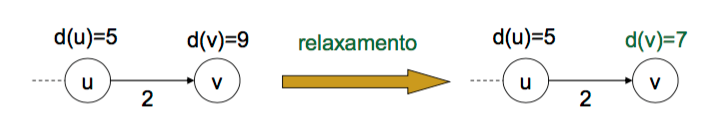
\includegraphics[width=0.9\textwidth]{img/relaxamento.png}
			\caption{Exemplo de um relaxamento de uma aresta. Fonte: \protect\url{http://wiki.icmc.usp.br/images/b/b4/7._1GrafosCaminhosLA(Graca).pdf}}
			\label{fig:relaxamento}
		\end{figure}
	\end{itemize}
\end{frame}

\begin{frame}{Variações deste Problema}
	\begin{itemize}
		\item Variações descritas até agora: 
		\begin{itemize}
			\item Caminho mais curto de uma única origem; e
			\item De todos para todos.
		\end{itemize}
	
		
		\item Mas além destes, é possível obter outras variantes deste problema sem perder sua essência. Seriam as outras variantes: 
		\begin{itemize}
			\item Caminho mais curto de destino único; e 
			\item Par único.
		\end{itemize}
	\end{itemize}
\end{frame}

\begin{frame}{Aplicações}
	\begin{itemize}
		\item Problemas de única origem:
		\begin{itemize}
			\item Problemas relacionados com sequências de decisões;
			\item Escolhas de itinerários ao longo de uma viagem;
			\item Traçado de uma estratégia em um problema de investimentos;
			\item Trata-se de decisões envolvendo alguma forma de custo a ser minimizado.
		\end{itemize}
		
		\bigskip
		
		\item Problema de todos para todos:
		\begin{itemize}
			\item Elaboração de uma tabela de distância entre todos os pares de cidades de um certa região para um atlas rodoviário.
		\end{itemize}
	\end{itemize}
\end{frame}


\end{document}
